\section{}
\begin{frame}
  \frametitle{Single Objective Optimization (SOP)}
  \begin{itemize}
    \item Optimize for one objective (goal)
    \item Search for global best solution
    \item Desired solution: global best
  \end{itemize}
  \vspace{1em}
  Example: Traveling Salesman Problem (TSP) with 5 cities, 1-5\\
  Objective: find shortest path\\
  Result: [2,5,1,4,3]
\end{frame}

\begin{frame}
  \frametitle{Multi Objective Optimization (MOP)}
  \begin{itemize}
    \item Optimize for several conflicting objectives (goals)
    \item No single ``best'' solution, instead number of solutions to chose from
    \item Desired solution: Optimal Pareto Front
  \end{itemize}
  \vspace{1em}
  Example: Traveling Salesman Problem (TSP) with 5 cities, 1-5\\
  Objectives: $f_1$) find shortest path with $f_2$) least costs\\
  Result: Pareto Front
  \begin{center}
    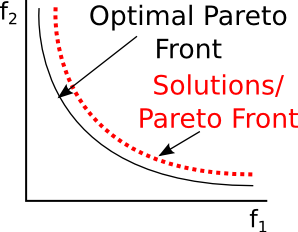
\includegraphics[width=30mm]{pareto-front-simple.png}
  \end{center}
\end{frame}

% \begin{frame}
%   \frametitle{Hadoop MapReduce and iterative problems}
%   MapReduce not suited for iterative problems:
%   \begin{itemize}
%     \item Data forwarding needs file system
%     \item Termination check needs separate component
%     \item Iterative problem must be mapped into map and reduce steps
%     \item Startup for map and reduce steps may take long time
%   \end{itemize}
%   \begin{center}
%     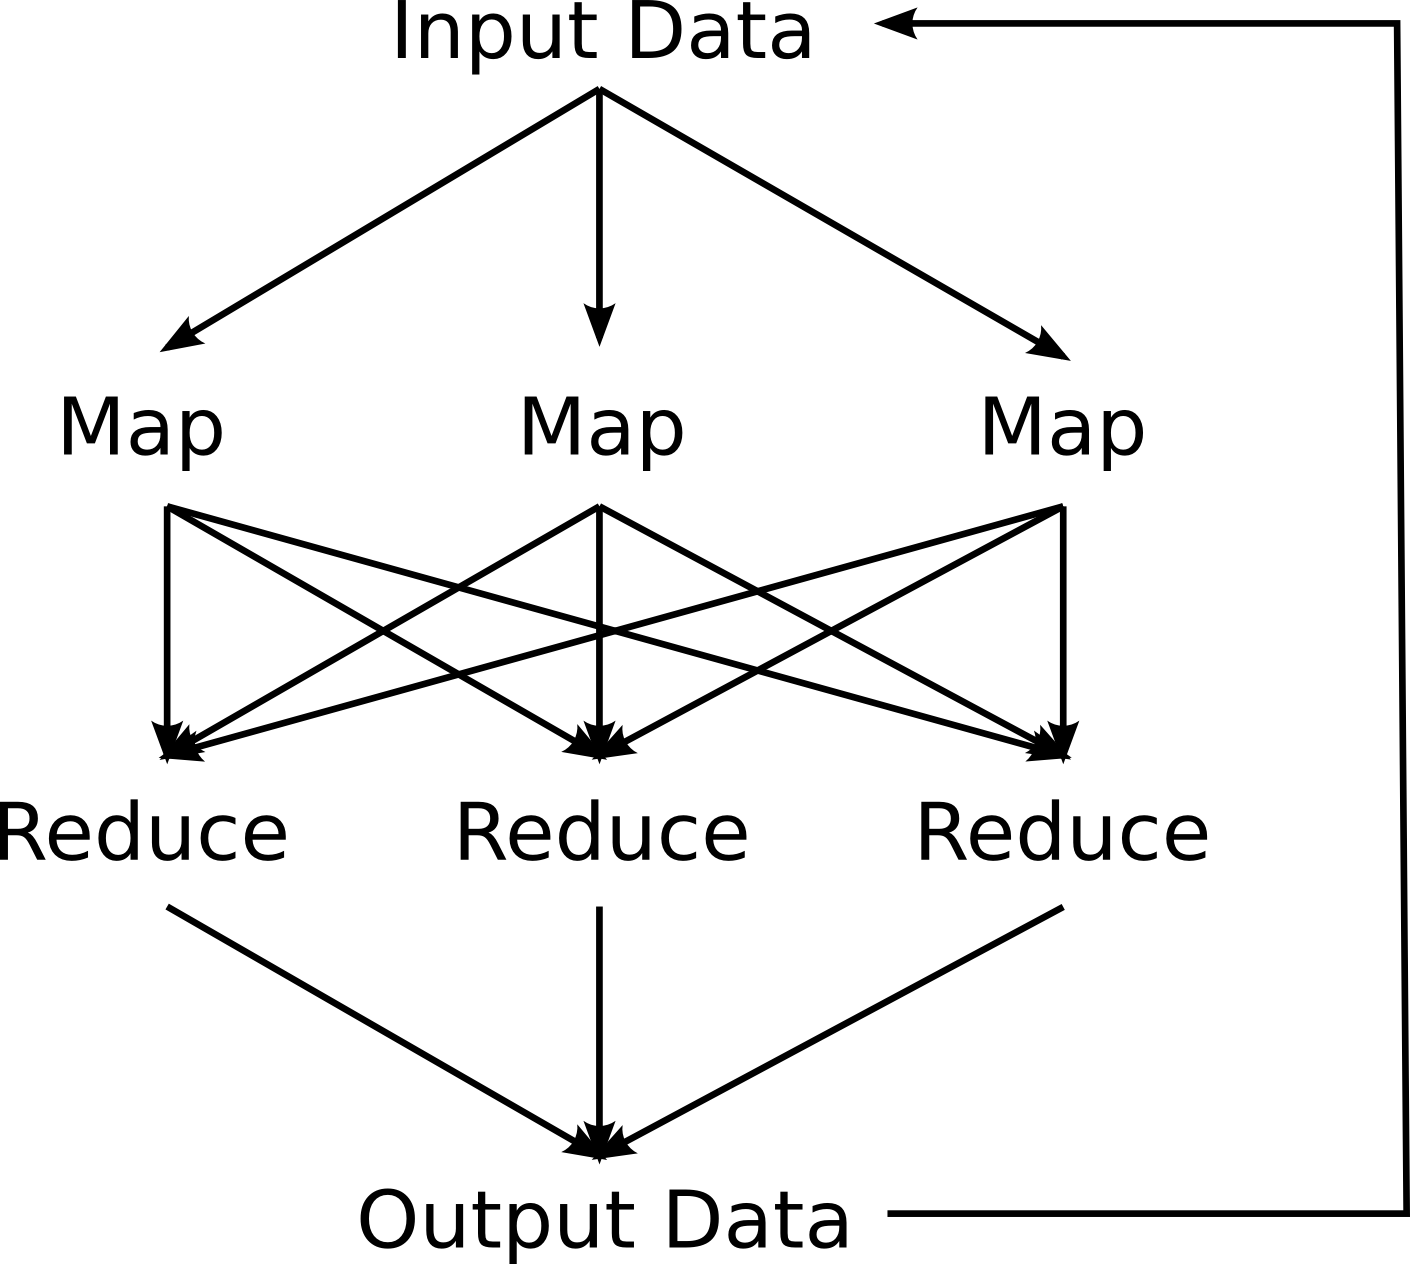
\includegraphics[width=30mm]{mapreduce.png}
%   \end{center}
% \end{frame}

\begin{frame}
  \frametitle{Biohadoop additional capabilities}
  \begin{itemize}
    \item Island model (parallelization model)
    \item Support for workers that don't run on Hadoop. Enables e.g. workers that run in browser or on mobile phone
    \item Custom communication facilities between master and worker
    \item Simple file system API
    \item Simple Config-Builders
    \item Development mode without Hadoop
  \end{itemize}
\end{frame}

\begin{frame}
  \frametitle{Island model}
  \begin{itemize}
    \item Multiple independent instances of optimization problems (e.g. GA) executed in parallel, instances are called islands
    \item Exchange solutions after certain intervals (integrate solutions from other islands)
    \item Important aspects:
    \begin{itemize}
      \item When to exchange solutions
      \item Which solutions to exchange
      \item How to merge solutions
    \end{itemize}
  \end{itemize}
  \begin{center}
    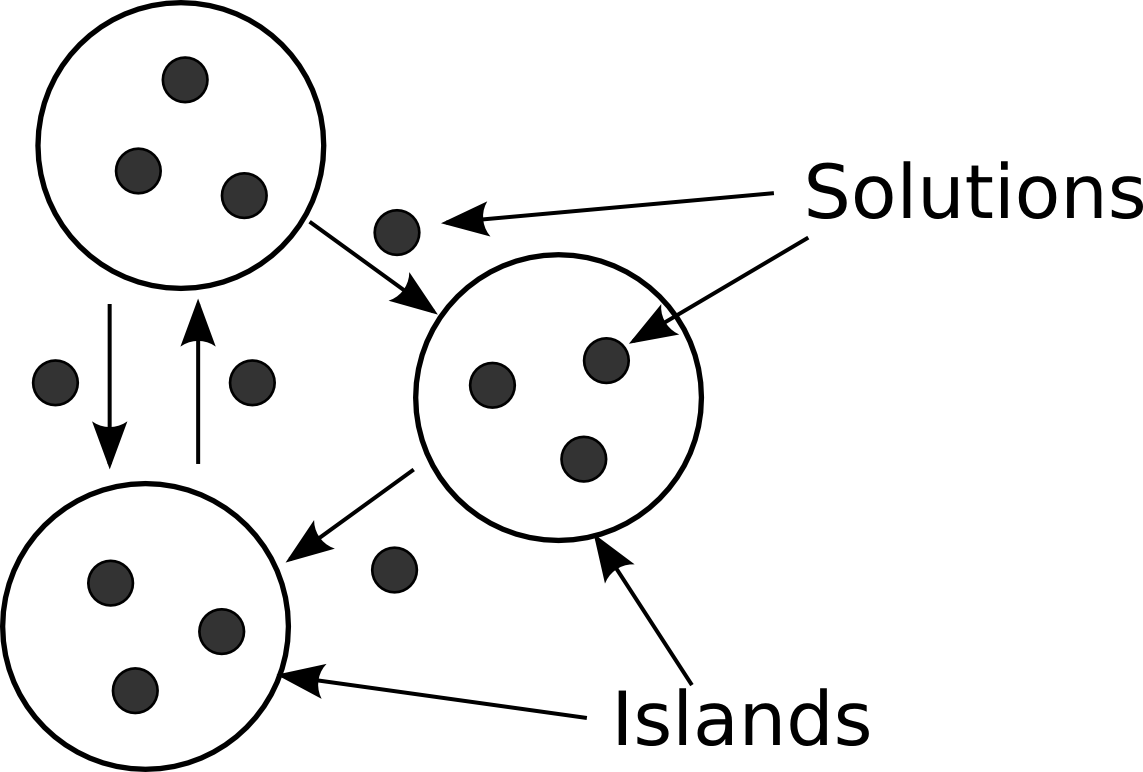
\includegraphics[width=30mm]{island-model-presentation.png}
  \end{center}
\end{frame}


\begin{frame}
  \frametitle{Docker-Biohadoop}
  \begin{itemize}
    \item Use of Docker containers
    \item Pre-build Hadoop environment
    \item Cluster simulation on single machine
    \item Play with Biohadoop
    \item \url{https://github.com/gappc/docker-biohadoop}, last access 05.03.2015
  \end{itemize}
\end{frame}

\begin{frame}[fragile]
  \frametitle{Biohadoop Java example}
  \texttt{Algorithm}
  \begin{lstlisting}[language=java,basicstyle=\tiny\ttfamily,breaklines=true,keywordstyle=\color{blue},stringstyle=\color{black},showstringspaces=false,frame=single]
public class ExampleAlgorithm implements Algorithm {
  @Override
  public void run(AlgorithmId algorithmId, Map<String, String> properties)
    String data = "Hello World!"
    TaskConfiguration<String> config = new TaskConfiguration<>(ExampleWorker.class, null);
    TaskFuture<String> future = TaskBroker.submit(data, config);
    String result = future.get();
  }
}
  \end{lstlisting}

  \texttt{Worker}
  \begin{lstlisting}[language=java,basicstyle=\tiny\ttfamily,breaklines=true,keywordstyle=\color{blue},stringstyle=\color{black},showstringspaces=false,frame=single]
public class ExampleWorker implements Worker<String, String, String> {
  @Override
  public String compute(String data, String initialData)
    return result + " - returned";
  }
}
  \end{lstlisting}
\end{frame}

\begin{frame}
  \frametitle{Unexpected execution time fluctuations}
  Large execution time differences found for same benchmarks/settings (up to \unit[50]{\%}):
  \begin{itemize}
    \item Hadoop has big influence on execution times: computation location, worker startup time
    \item Other influences: Network, RAM, CPU caches, Java Just In Time compiler (JIT), Java libraries (e.g. communication), OS...
  \end{itemize}
  \vspace{1em}
  $\rightarrow$ VERY difficult to find reasons for performance problems in distributed systems - \textbf{better tool support needed}
\end{frame}

\begin{frame}
  \frametitle{Improvements}
  \begin{itemize}
    \item Web based interface to interact with Service
    \item Accelerate communication (reduce network overhead)
    \item Implement batch communication
    \item Provide API for Worker-to-Worker communication (enable different computation models)
    \item Implement distributed caching
    \item Provide API for multi-threading workers
    \item Provide metrics
  \end{itemize}
\end{frame}

\begin{frame}
  \frametitle{Web based interface}
  \begin{itemize}
    \item Manage authentication and authorization
    \item Provide interface to:
    \begin{itemize}
      \item Upload Biohadoop based algorithm
      \item Upload data
      \item Retrieve results
      \item Start/stop/monitor executions
    \end{itemize}
  \end{itemize}
\end{frame}
